\documentclass[default]{beamer}
\setbeamertemplate{navigation symbols}{}

\usetheme{CambridgeUS}
%\useoutertheme{infolines}
\usecolortheme{beaver}

\usepackage[utf8]{inputenc}					% Выбор языка и кодировки
\usepackage[english, russian]{babel}	% Языки: русский, английский
\usepackage{csquotes}

\usepackage{tikz}
\usetikzlibrary{arrows,shapes,calc}
\everymath{\displaystyle}
\tikzstyle{every picture}+=[remember picture]

\usepackage{animate}
\usepackage{fp}
\usepackage{textpos}

\usepackage[
	language=auto,
	autolang=other,
	backend=biber,
	style=authortitle,
	sorting=ydnt,
	maxbibnames=5
]{biblatex}
\addbibresource{panov_sait2017.bib}
				
\DeclareSourcemap{
	\maps[datatype=bibtex, overwrite]{
		\map{
			\step[fieldset=langid, fieldvalue=english]
			\step[fieldset=doi, null]
			\step[fieldset=issn, null]
			\step[fieldset=isbn, null]
			\step[fieldset=url, null]
			\step[fieldsource=language, fieldset=langid, origfieldval]
		}
	}
}
\DeclareBibliographyDriver{std}{%
	\usebibmacro{bibindex}%
	\usebibmacro{begentry}%
	\usebibmacro{author/editor+others/translator+others}%
	\setunit{\labelnamepunct}\newblock
	\usebibmacro{title}%
	\newunit\newblock
	\usebibmacro{maintitle+booktitle}
	\newunit\newblock
	\usebibmacro{journal}%
	\newunit\newblock
	\usebibmacro{date}%
	\newunit\newblock
	\usebibmacro{finentry}
}
\DeclareBibliographyAlias{article}{std}
\DeclareBibliographyAlias{book}{std}
\DeclareBibliographyAlias{inproceedings}{std}
\DeclareBibliographyAlias{incollection}{std}

\graphicspath{{../../images/}} 			% Пути к изображениям

\makeatletter
\setbeamertemplate{footline}
{
	\leavevmode%
	\hbox{%
		\begin{beamercolorbox}[wd=.333333\paperwidth,ht=2.25ex,dp=1ex,center]{author
				in head/foot}%
			\usebeamerfont{author in
				head/foot}\insertshortauthor~~\beamer@ifempty{\insertshortinstitute}{}{(\insertshortinstitute)}
		\end{beamercolorbox}%
		\begin{beamercolorbox}[wd=.333333\paperwidth,ht=2.25ex,dp=1ex,center]{title in
				head/foot}%
			\usebeamerfont{title in head/foot}\insertshorttitle
		\end{beamercolorbox}%
		\begin{beamercolorbox}[wd=.333333\paperwidth,ht=2.25ex,dp=1ex,right]{date in
				head/foot}%
			\usebeamerfont{date in head/foot}\insertshortdate{}\hspace*{1em}
			\insertframenumber{}\hspace*{2ex} 
		\end{beamercolorbox}
	}%
	\vskip0pt%
}

\addtobeamertemplate{frametitle}{}{
	\begin{textblock*}{100mm}(\textwidth-35pt,-20pt)
		
\includegraphics[width=1.5cm]{misc/logos/frccsc.png}
	\end{textblock*}
}

\newcommand{\predmatr}[3]{
	\node[ell, rectangle, minimum height = 15, minimum width = 7.5]  at (#1 pt,#2 pt) {}; 
	\node[ellf, rectangle, minimum height = 15, minimum width = 7.5] at (#1+7.5 pt,#2 pt) {};
	\node[minimum height = 15, minimum width = 15] (#3) at (#1+3.3pt,#2 pt) {};
	\draw[ell] (#1+7.5 pt,#2+7.5 pt) -- (#1 +7.5 pt,#2-7.5 pt);
}
\renewcommand*{\bibfont}{\tiny}
\setlength\bibitemsep{-5pt}

\begin{document}
	
	\title[Обучение перемещению]{Автоматическое формирование правил перемещения с использованием обучения с подкреплением}
	\author[Панов и Суворов]{Александр Панов и Роман Суворов}
	\institute[ФИЦ ИУ РАН]{Федеральный исследовательский центр <<Информатика и управление>>\\Российской академии наук}
	\date[16 июня -- САИТ 2017]{16 июня -- САИТ 2017\\г.~Светлогорск, Россия} 
		
	\begin{frame}
		\titlepage
		\centering
		\includegraphics[width=100pt]{misc/logos/ras.png} \hspace{10pt}
		
\includegraphics[width=80pt]{misc/logos/frccsc.png}
	\end{frame}

	\section{Введение}
	\subsection{Знаковая картина мира}

	\begin{frame}
		\frametitle{Картина мира субъекта деятельности}
		\scriptsize
		\onslide<1->{
			Картина мира субъекта деятельности - это представления субъекта о внешней среде, о своих собственных характеристиках, целях, мотивах, о других субъектах и операции (произвольные и непроизвольные), осуществляемые на основе этих представлений.
		}
		\onslide<2->{
			\par\smallskip
			Элементом картины мира является знак:
			\begin{itemize}
				\item в смысле культурно-исторического подхода Выготского-Лурии,
				\item выполняющий функции в соответствии с теорией деятельности Леонтьева.
			\end{itemize}
		}
		\onslide<3->{
			\begin{columns}
				\begin{column}{0.4\textwidth}
					\centering
					\includegraphics[width=0.6\textwidth]{signs/ru/sign_color_book_ru}
				\end{column}
			}
		\onslide<4->{
				\begin{column}{0.6\textwidth}
					\begin{columns}
						\begin{column}{0.5\textwidth}
							\centering
							\includegraphics[width=\textwidth]{misc/phisio/ivan_cyrc}
						\end{column}
						\begin{column}{0.5\textwidth}
							\centering
							\includegraphics[width=\textwidth]{misc/phisio/workspace}
						\end{column}
					\end{columns}
				\end{column}
			\end{columns}
			В пользу существования такой структуры свидетельствуют:
			\begin{itemize}
				\item нейрофизиологические данные (Эдельман, Иваницкий, Маунткастл и др.),
				\item другие психологические теории (например, трехкомпонентная модель Станович).
			\end{itemize}
			\vspace{-5pt}
			\nocite{*}
			\printbibliography[keyword={sign}, resetnumbers=true]
		}
	\end{frame}
				
	\begin{frame}
		\frametitle{Моделирование картины мира}
		\begin{columns}
			\begin{column}{0.5\textwidth}
				\centering
				\includegraphics[width=0.7\textwidth]{causnet/caus_matr_ru}
				
				
			\end{column}
			\begin{column}{0.5\textwidth}
				\centering
				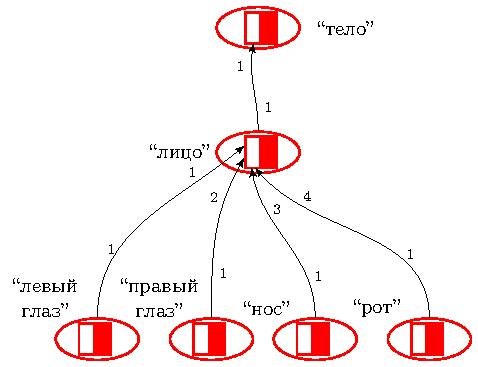
\includegraphics[page=1,width=0.7\textwidth]{examples/causnet/caus_net_colored}
			\end{column}
		\end{columns}
		\begin{columns}
			\begin{column}{0.5\textwidth}
				\centering
				\includegraphics[width=0.7\textwidth]{signnet/signs_net}
			\end{column}
			\begin{column}{0.5\textwidth}
				Модель картины миры (семиотическая сеть):
				\[\Omega=\langle W_p, W_m, W_a, R_n, \Theta \rangle\]
				
				\vspace{-5pt}
				\nocite{*}
				\printbibliography[keyword={signmodel}, resetnumbers=true]
			\end{column}
		\end{columns}
	\end{frame}

	\subsection{Применение модели}
	
	\begin{frame}
		\frametitle{Применение модели}
		\vspace{-5pt}
		\footnotesize
		\begin{columns}
			\begin{column}{0.43\textwidth}
				\begin{itemize}
					\item Моделирование когнитивных функций и построение моделей, объясняющих психологические феномены.
					\item Алгоритмы синтеза плана поведения (алгоритмы MAP, MultiMAP, GoalMAP).
					\item Решение проблемы символизации.
					\item Построение картины мира субъекта на основе текстов.
					\item Генерация сообщений на основе картин мира определенного типа (виртуальные ассистенты).
					\item Построение многоуровневых архитектур управления.
				\end{itemize}
				
			\end{column}
			\begin{column}{0.57\textwidth}
				\includegraphics[width=\textwidth]{agent-schemas/ru/architecture}
			\end{column}
		\end{columns}
		\vspace{-5pt}
		\nocite{*}
		\printbibliography[keyword={strl}, resetnumbers=true]
	\end{frame}

	\begin{frame}
		\frametitle{Проблема символизации в робототехнике}
		
		\begin{columns}
			\begin{column}{0.43\textwidth}
				\includegraphics[width=\textwidth]{misc/agents/turtlebot-2.jpg}
				
				
			\end{column}
			\begin{column}{0.57\textwidth}
				Как на основе сенсомоторной информации сформировать символы, концепты, понятия, знаки:
				\begin{itemize}
					\item symbol grounding problem - Harnad, 1990; Barsalou, 1999, 2008; Sun, 2013;
					\item anchoring problem - Vernon, 2014; Карпов, 2016;
					\item семиотические схемы - Roy, 2005;
					\item потоковая модель DyKnow - Heintz, 2010;
					\item концепторы - Jaeger, 2014;
					\item система SemLinks - Butz, 2016, 2017.
				\end{itemize}
			\end{column}
		\end{columns}
	\end{frame}

	\begin{frame}
		\frametitle{Обучение правилам перемещения}
		\footnotesize
		Особенность задачи:
		\begin{itemize}
			\item Использование обучения с подкреплением для формирования компонент знаковой картины миры.
			\item В качестве знаний о среде агент использует <<сырую>> сенсорную информацию.
			\item Задача агента - в результате обучения сформировать картину мира: некоторое понятийное описание среды, включающее дискретные правила действования в нем.
			\item Более широкая постановка - задача совместного планирования в пространстве с распределением ролей и коммуникацией.
		\end{itemize}
		\begin{center}
			\scalebox{0.35}{
				\animategraphics{12}{examples/plan/slides_colored}{}{}			
			}
		\end{center}
	\end{frame}


	\section{Постановка задачи}
	\subsection{Обучение с подкреплением}
	\begin{frame}
		\frametitle{Обучение с подкреплением: общая постановка}
		\textbf{Основные понятия:}
		\begin{itemize}
			\item $a_t: s_t\rightarrow s_{t+1}$ - действия агента в среде,
			\item $r_t$ - вознаграждение, получаемое агентом от среды,
			\item цель агента - максимизация суммарного вознаграждения $R=\sum\limits_{t}{{{\gamma }^{t}}}{{r}_{t}}$, $0<\gamma\le 1 $,
			\item $\pi :S\rightarrow A$ - стратегия агента, учитывающая предыдущий опыт и необходимость исследования среды ($\epsilon$-жадный метод).
		\end{itemize}
	
		\textbf{Способы решения:}
		\begin{itemize}
			\item Если известны $T(s_t,a_t,s_{t+1})$ и $r(s_t,a_t)$, то это задача, основанная на модели, решение \textit{уравнения Беллмана}.
			\item Оценка функции полезности $V(s)=\mathbf{E}[R|s,\pi]$ или функции полезности действия $Q(s,a)=\mathbf{E}[R|s,a,\pi]$.
		\end{itemize}
	\vspace{-5pt}
	\nocite{*}
	\printbibliography[keyword={rlearn}, resetnumbers=true]
	\end{frame}
	
	\begin{frame}
		
		\frametitle{Обучение с подкреплением: правила перемещения}
		\begin{columns}
			\begin{column}{0.7\textwidth}
				\begin{itemize}
					\item $E=(M,G)$ - среда, где $M$ - карта местности, $G(p_s,p_f)$ - алгоритм генерации вознаграждения,
					\item $a_t=p_t\rightarrow p_{t+1}$ - действия агента по перемещению,
					\item $s_t\in R^{(2d)^2}$ - наблюдения агента (сенсорная информация).
				\end{itemize}
			\end{column}
			\begin{column}{0.3\textwidth}
				\centering
				\includegraphics[width=\textwidth]{examples/path/map1}
			\end{column}
		\end{columns}
		\vspace*{10pt}
		Пусть ${{Q}^{*}}({{s}_{t}},{{a}_{t}})={{\max }_{\pi }}\mathbf{E}[R|{{s}_{t}},{{a}_{t}},\pi ]$ - оптимальная функция полезности, тогда с учетом определения $R$ \tikz[baseline] \node[coordinate] (n1) {}; получаем следующее уравнение Беллмана:
		\begin{equation*}
			Q^*(s,a)=\mathbf E_{s_t\sim E}\left[
			\tikz[baseline]{
				\node[fill=blue!20,anchor=base] (t1)
				{$r_t+\gamma\max_{a_t}Q^*(s_t,a_t)$};
			}
			|s,a \right]
		\end{equation*}
		\begin{tikzpicture}[overlay]
			\path[->] (n1.south) edge [bend left, out = 50] (t1);
		\end{tikzpicture}
	\end{frame}

	\begin{frame}
		\frametitle{Обучение с подкреплением: аппроксимация}
		
		Для решения итерационными методами уравнения Беллмана используют различные аппроксимации функции ${{Q}^{*}}(s,a)$: $Q(s,a;\theta )\approx {{Q}^{*}}(s,a)$. 
		\par\medskip
		В процессе обучения происходит настройка параметров $\theta$ в результате минимизации функции потерь $L(\theta)$:
		
		\begin{multline*}
			L_i(\theta_i)=\mathbf E_{s,a\sim\rho(\cdot)}\left[(
			\tikz[baseline]{
				\node[fill=blue!20,anchor=base] (t1)	
				{$y_i$};
			}
			-Q(s,a;\theta_i))^2\right],\\
			y_i=
			\tikz[baseline]{
				\node[fill=green!20,anchor=base] (t2)
				{$\mathbf E_{s_t\sim E}\left[r_t+\gamma\max_{a_t}Q(s_t,a_t;\theta _{i-1})|s,a \right]$};
			}
		\end{multline*}
		
		\begin{multline*}
			{{\nabla }_{{{\theta }_{i}}}}{{L}_{i}}({{\theta }_{i}})={{\mathbf{E}}_{s,a\sim \rho (\cdot );{{s}_{t}}\sim E}}\left[ \left( {{r}_{t}}+\gamma {{\max }_{{{a}_{t}}}}Q({{s}_{t}},{{a}_{t}};{{\theta }_{i-1}}) \right. \right.- \\ 
			\left. \left. -Q(s,a;{{\theta }_{i}}) \right){{\nabla }_{{{\theta }_{i}}}}Q(s,a;{{\theta }_{i}}) \right].
		\end{multline*}
			

		\begin{tikzpicture}[overlay]
			\path[<-] (t1.north) edge [bend left,in = 120] (t2);
		\end{tikzpicture}
	\end{frame}

	\begin{frame}
		\frametitle{Обучение с подкреплением: переигровки}
		\begin{itemize}
			\item Эпизод - это набор действий агента и реакций среды на перемещения от начального положения до конечно, либо до достижения максимального количества действий $N_a$,
			\item $e_t=(s_t,a_t,r_t,s_{t+1})$ - прецедент сохраняется в память агента $D$,
			\item обучение идет по некоторой случайной выборке $e$ \tikz[baseline] \node[coordinate] (n1) {}; из памяти 
		\end{itemize}
	
		\begin{equation*}
			D=\left\{ e_1, 
				\tikz[baseline]{
					\node[fill=blue!20,anchor=base] (t1)
					{$e_2$};
				}
			,\dots, 
				\tikz[baseline]{
					\node[fill=blue!20,anchor=base] (t2)
					{$e_i$};
				}
			,e_{i+1},\dots e_j,
				\tikz[baseline]{
					\node[fill=blue!20,anchor=base] (t3) 
					{$e_{j+1}$};
				}
			,\dots \right\}
		\end{equation*}
		\begin{tikzpicture}[overlay]
			\path[->] (t1) edge [bend left, out = 50, in=-150] ([xshift=-10pt,yshift=-2pt]n1);
			\path[->] (t2) edge [bend left, out = 40, in=-130] ([xshift=-6pt,yshift=-2pt]n1);
			\path[->] (t3) edge [bend left, out = 30, in=-90] ([xshift=-2pt,yshift=-2pt]n1);
		\end{tikzpicture}
		\begin{itemize}
			\item одно действие можно использовать несколько раз $\rightarrow$ расширяем выборку, устраняем корреляции соседних состояний.
		\end{itemize}
	\end{frame}
	
	\begin{frame}
		\frametitle{Генерация вознаграждения}
		
		Для расчета функции вознаграждения использовали следующий алгоритм:
		\begin{equation*}
			G(s,g,t)=\begin{cases}
				\alpha_{opt}r_t^{opt}+\alpha_{rat}r_t^{rat}+\alpha_{euq}r_t^{euq}, & p_t\leftarrow 0,\\
				r^{obs}, & p_t\leftarrow 1,\\
				r^{tar}, & p_t=g,
			\end{cases}
		\end{equation*}
		где 
		\begin{itemize}
			\item $\sum\alpha_i=1$ - нормировка,
			\item $r_t^{opt}=l_t-l_{t-1}$ - изменение оптимального расстояния,
			\item $r_t^{rat}=e^{-l_t/l_0}$ - штраф за отклонение от цели,
			\item $r_t^{euq}=|p_t-g|-|p_{t-1}-g|$ - регуляризатор для спрямления пути.
		\end{itemize}
	\end{frame}

	\subsection{Архитектуры регрессоров}
	\begin{frame}
		\frametitle{Гетерархическая каузальная сеть}
		Биологически правдоподобная модель обучения (формирования компонента знака) включает:
		\begin{itemize}
			\item сканирующее рецептивное поле - формирование паттерна,
			\item пространственный группировщик (кластеризация паттернов online K-means),
			\item временной группировщик (аггломеративная кластеризация $\rightarrow$ марковские цепи).
		\end{itemize}
		\centering
		\vspace*{-3pt}
		\includegraphics[width=0.39\textwidth]{misc/mpf/hawkins_htm.jpg}
	\end{frame}

	\begin{frame}
		\frametitle{Нейросетевые архитектуры}
		В работы мы проводили эксперименты с различными нейронными сетями:
		\begin{enumerate}
			\item $Ag_1$ - <<мелкая>> полносвязная нейронная сеть,
			\item $Ag_2$ - сверточная сеть средней глубины с полносвязными выходным слоем,
			\item $Ag_3$ - глубокая сеть, состоящая из блоков Inception.
		\end{enumerate}
		\centering
		\includegraphics[width=0.8\textwidth]{examples/path/neural_arch.png}
	\end{frame}

	\section{Эксперименты}
	\begin{frame}
		\frametitle{Карты, пути, параметры}
		Самый успешный наборов параметров:
		\begin{itemize}
			\item $N_{ep}\sim 3000$ - количество эпизодов, $N_a=100$ - ограничение по шагам, $d=20$ - радиус видимости агента,
			\item $\alpha_{opt}=0.8,\alpha_{rat}=0.1$ - значения коэффициентов вознаграждения,
			\item $r^{obs}=-4,r^{tar}=10$ - значения параметров вознаграждения,
			\item $N_e=10$ - размер памяти $D$,
			\item $\gamma=4$ - дисконтирующий множитель при расчете вознаграждения.
		\end{itemize}
		\centering
		\includegraphics[width=0.35\textwidth]{examples/path/path_example.png}
		\includegraphics[width=0.35\textwidth]{examples/path/path_example_2.png}
	\end{frame}

	\begin{frame}
		\frametitle{Cходимость процесса обучения}
		\begin{columns}
			\begin{column}{0.65\textwidth}
				\centering
				\includegraphics[width=\textwidth]{examples/path/batch_full_smoothed.png}
				\vspace*{-10pt}
				\includegraphics[width=\textwidth]{examples/path/run_episodes_smoothed.png}
			\end{column}
			\begin{column}{0.35\textwidth}
				Мы использовали две метрики качества:
				\begin{itemize}
					\item $M_p$ - отношение длины пути, построенного агентом, к оптимальному,
					\item $M_r$ - отношение суммарного вознаграждения к максимальному.
				\end{itemize}
			\end{column}
		\end{columns}
		
		
	\end{frame}

	\begin{frame}
		\centering
		\Huge
		Спасибо за внимание!
		\normalsize
		\par\bigskip
		\par\bigskip
		\par\bigskip
		pan@isa.ru
		\par\bigskip
		ФИЦ ИУ РАН, лаб. 0-2
	\end{frame}			
\end{document}
	
	
